\documentclass[parskip=full, numbers=noenddot]{scrbook}

% starts new page with new section
\usepackage{titlesec}
\newcommand{\sectionbreak}{\clearpage}

% makes abstract possible in scrbook
\newenvironment{abstract}%
{\cleardoublepage\null \vfill\begin{center}%
    \bfseries \abstractname \end{center}}%
    {\vfill \null}

% language
\usepackage[english]{babel}
\usepackage[utf8]{inputenc}
\usepackage{csquotes}
\usepackage{url}
\usepackage[version=4]{mhchem}
\usepackage{siunitx}
\DeclareSIUnit\molar{\mole\per\cubic\deci\metre}
\DeclareSIUnit\Molar{\textsc{m}}
\DeclareSIUnit\calorie{cal}

% citations
\usepackage[
  natbib=true,
  backend=biber,
  doi=true,
  isbn=false,
  url=false,
  date=year,
  style=apa,
  citestyle=apa]{biblatex}
\addbibresource{dissertation.bib}
\usepackage{varioref}

% floats
\usepackage{graphicx}
  \graphicspath{ {./graphics/} }
\usepackage{subcaption}
\usepackage{tabularx}
  \newcolumntype{L}{>{\raggedright\arraybackslash}X}
\usepackage{booktabs}
\usepackage{pgfplotstable}
\usepackage{tikz}
\usetikzlibrary{shapes, arrows}
\tikzstyle{reagent} = [trapezium, trapezium left angle=70, trapezium right angle=110, text width=7em, text centered, draw=black, fill=blue!20]
\tikzstyle{process} = [rectangle, text width=7em, text centered, draw=black, fill=orange!30]
\tikzstyle{cloud} = [draw, ellipse]
%\tikzstyle{arrow} = [thick,->,>=stealth]
\tikzstyle{line} = [draw, -latex']

\title{Sequence Preferences of the Nucleosome and PCR Enzymes}
\author{Candidate number XXXXX}

\begin{document}

%% NOTE ABOUT KMER PLOTS: currently I've added the PNG images so that the report isn't 60 MB.  Near the end I'll replace them with the corresponding PDF images.
%% Also I'm supposed to make the spacing between lines 1.5x but still can't bring myself to do it, it looks so pleasing atm

\frontmatter

\maketitle
% Will deal with the intricacies of the cover pages at the very end.

\begin{abstract}
% problem, approaches (in outline), major findings. make main points absolutely clear. aim for 200-250 words
  
  Nucleosome positioning on the genome closely correlated to gene expression.  CpG methylation has been found to disfavour nucleosomes \emph{in vivo}, it is not clear how this preference can be explained.  Furthermore, the effects of non-CpG methylation have not been characterised.  In the first part of this study, we use  nucleosome EMSA-SELEX to select oligonucleotides that bind to histone octamers, and characterised nucleosome's sequence preferences for methylated DNA.  This approach not only confirmed existing `rules' for nucleosome positioning: there was a sequence periodicity of 10 base pairs, TA occurred out of phase with GC, and stretches of adenines disfavoured nucleosome positioning.  But also, we found that cytosine methylation aligns the phases of dinucleotides harbouring cytosines compared to unmethylated DNA.  % Finally, CpG-methylated and half-C-methylated DNA containing A/T-rich nucleotide 9-mers were found to disfavour nucleosome positioning.
  The new ‘rules’ regarding methylated C are useful for more precise prediction of gene regulations.

PCR is indispensable in most workflows of next-generation sequencing. However, PCR biases considerably undermines the reliability of sequencing results.  To better understand and model such PCR biases, in the second part of the project, we studied the effects from PCR cycles, enzyme identity, bottlenecking, template concentration, DNA purification, and reagent vendors.  Our findings suggest that DreamTaq, Phusion, Phire, and Q5 DNA polymerases had weak biases towards A and T, with Phusion exhibiting the least bias and Phire the greatest.  Compared to the intrinsic biases of the enzymes, the effects were minor for the bottlenecking effect, DNA purification by AMPure beads, and for the vendors of DNA polymerase and dNTPs.  Such information would help develop an explicit model accounting for PCR bias, thus allowing us to alleviate its effects on the analysis of sequencing data.
 
\end{abstract}

\tableofcontents

\chapter*{List of Abbreviations}
\label{ch:abbrev}

\begin{description}
\item [bp] base pair
\item [dCTP] deoxycytidine triphosphate
\item [dNTP] deoxynucleotide triphosphate
\item [EMSA] electrophoretic mobility shift assay
\item [FFT] fast Fourier transform
\item [M.SssI] CpG methyltransferase isolated from \emph{E. coli} containing the methyltransferase gene from \emph{Spiroplasma} sp.\ strain MQ1
\item [MNase] micrococcal nuclease
\item [PCR] polymerase chain reaction
\item [SELEX] systematic evolution of ligands by exponential enrichment
\item [TBE] tris-borate EDTA
\end{description}

\mainmatter

\chapter{Nucleosome EMSA-SELEX}
\label{ch:emsaselex}

\section{Introduction}
\label{sec:emsaselex_intro}

\subsection{Physiological importance of the nucleosome}
\label{ssec:emsaselex_intro_importance}

Eukaryotes package their DNA into chromatin through a series of coiling steps.  The fundamental repeating unit of chromatin is the nucleosome, which consists of a histone octamer with 147 base pairs (bp) of DNA wrapped around it.  Nucleosome positioning is an important determinant in gene expression because nucleosomes inhibit binding of DNA-binding proteins to DNA.  Specifically, nucleosome positioning inhibits transcription by preventing RNA polymerase from accessing chromatin, and prevent binding of transcription factors to regulatory elements.

\subsection{Nucleosome sequence preferences}
\label{ssec:emsaselex_intro_seqpref}

For a given 147-bp DNA sequence, the affinity of the histone octamer to it can vary over more than three orders of magnitude.  This is mainly because the nucleotide sequence and the methylation state of nucleotides affect the physical flexibility (`bendability') of DNA in certain directions, which is required for the wrapping of DNA around histone octamers.

The dinucleotide sequences AA, AT, and TA confer high bendability to DNA.  Therefore, they are situated on the phase of the helical repeat that directly interacts with the histone octamer, with a periodicity of approximately 10 bp \citep{struhl_determinants_2013}.  GC dinucleotides also occur periodically, but out of phase with the aforementioned dinucleotides.  These preferences were confirmed by a yeast-based genome-wide assay based on MNase-seq \citep{segal_genomic_2006}.  Experiments with synthetic DNA in SELEX (systematic evolution of ligands by exponential enrichment) \citep{lowary_new_1998} have elucidated more rules for nucleosome positioning.  The `pentameric TG' sequence -- [(A or T)3NN(G or C)3NN]n -- has a very high affinity for the histone octamer, consistent with how AT-rich and GC-rich units confer flexibility of DNA.  `Phased TATA' sequences possessing multiple phased CTA trinucleotides also exhibit high affinity.

In contrast, the homopolymeric sequences poly(dA:dT) and poly(dG:dC) form stiff structures that inhibit nucleosome formation.  These sequences are enriched in linker DNA between nucleosomes.  Poly(dA:dT) sequences are also enriched in promoters, in particular that of \emph{Saccharomyces cerevisiae} \citep{struhl_determinants_2013}.  Depletion of nucleosomes at promoters on artificial chromosomes based on \emph{S. cerevisiae} genomic regions was shown to be dependent on the number and length of poly(dA:dT) sequences \citep{hughes_functional_2012}.

Additionally, DNA methylation disfavours nucleosome positioning \emph{in vivo}, as it increases the rigidity of DNA \citep{huff_dnmt1-independent_2014}.  Specifically, multiple tracts of methylated CpG islands makes DNA have lower rise and twist along with higher roll values, thus making the DNA stiffer \citep{rao_systematic_2018, perez_impact_2012}.  However, the negative correlation between nucleosome occupancy and DNA methylation varies according to the genomic location.  For example, this negative correlation holds for CTCF regions, but not at promoters \citep{kelly_genome-wide_2012}.

\subsection{Purpose of this study}
\label{ssec:emsaselex_intro_why}

CpG methylation is the predominant chemical modification of eukaryotic DNA, playing roles in gene regulation and physiology. Although CpG methylation was shown to affect in vivo nucleosome positioning \citep{kelly_genome-wide_2012}, it is not clear whether such effects are due to biochemical affinity change or due to secondary effects from other proteins.  Furthermore, CH methylation (non-CpG methylation) also regulates development of stem cells and neurons \citep{guo_distribution_2014}; however, little is known about the effects of CH methylation on sequence preferences of nucleosomes.

SELEX is the most direct biochemical approach to identify the DNA sequences preferred for nucleosome positioning.  Unlike MNase-seq, SELEX employs a random DNA library, which has greatly higher complexity than genomic sequences and a more homogeneous background sequence distribution.  Previous work \citep{lowary_new_1998} employed SELEX in uncovering sequence-based rules for nucleosome positioning, but analysis was limited by the capacity of sequencing.  This project extended on their study by sequencing a more complex library to a higher depth, allowing identification of signals with higher information content.

In this project, I aimed to study the sequence specificity of the nucleosome on methylated and non-methylated DNA.  I conducted four cycles of nucleosome EMSA SELEX using random DNA methylated at different level as input libraries, using affinity to the histone octamer as part of the evolution process.  After sequencing, the periodicity and amplitudes of mononucleotides and dinucleotides in all DNA libraries were characterised using fast Fourier transform \citep{lowary_new_1998, zhu_interaction_2018}.  Additionally, I assessed sequence biases by assessing \emph{k}-mer distributions.

\section{Results}
\label{sec:emsaselex_results}

\begin{figure}[htpb]
  \hspace*{-1cm}
\begin{tikzpicture}[node distance=2cm]
  %% nodes
  % input lib and amplification
  \node [reagent] (lig147) {lig147};
  \node [cloud, below of=lig147] (circle01) { };
  \node [process, below of=circle01] (amphalfmc) {Amplify with methyl-C + C};
  \node [process, left of=amphalfmc, xshift=-6cm] (amp) {Amplify};
  \node [process, right of=amphalfmc, xshift=2cm] (ampallmc) {Amplify with methyl-C};
  \node [reagent, below of=amp] (plain01) {Plain DNA};
  % amplified libraries (broadly)
  \node [reagent, below of=plain01] (plain02) {Plain DNA};
  \node [reagent, below of=amphalfmc, yshift=-2cm] (half-c-methylated) {Half-C-methylated};
  \node [reagent, below of=ampallmc, yshift=-2cm] (all-c-methylated) {All-C-methylated};
  \node [reagent, left of=half-c-methylated, xshift=-2cm] (cpg-methylated) {CpG-methylated};
  \node [process, above of=cpg-methylated, yshift=-0.75cm] (cpg) {CpG methylation};
  % nucleosome reconstitution
  \node [process, below of=half-c-methylated] (reconstitution) {Nucleosome reconstitution};
  % reconstituted nucleosomes
  \node [reagent, below of=reconstitution] (half-c-methylated-nuc) {Half-C-methylated nucleosome};
  \node [reagent, left of=half-c-methylated-nuc, xshift=-6cm] (plain-dna-nuc) {Plain DNA nucleosome};
  \node [reagent, left of=half-c-methylated-nuc, xshift=-2cm] (cpg-methylated-nuc) {CpG-methylated nucleosome};
  \node [reagent, right of=half-c-methylated-nuc, xshift=2cm] (all-c-methylated-nuc) {All-C-methylated nucleosome};
  % emsa
  \node [process, below of=half-c-methylated-nuc] (emsa) {EMSA and elute};
  % eluted
  \node [reagent, below of=emsa] (half-c-methylated-bub) {Half-C-methylated DNA bound and unbound};
  \node [reagent, left of=half-c-methylated-bub, xshift=-6cm] (plain-dna-bub) {Plain DNA bound and unbound};
  \node [reagent, left of=half-c-methylated-bub, xshift=-2cm] (cpg-methylated-bub) {CpG-methylated DNA bound and unbound};
  \node [reagent, right of=half-c-methylated-bub, xshift=2cm] (all-c-methylated-bub) {All-C-methylated DNA bound and unbound};
  % the bottom bit
  \node [cloud, below of=half-c-methylated-bub] (circle02) { };
  \node [process, below of=circle02] (barcoding) {Barcoding and sequencing};
  %% edges
  % lig147 to circle01
  \path [line] (lig147) -- (circle01);
  % between circle01 and amped libs
  \path [line] (circle01) --++ (0cm,-1cm) -| (amp);
  \path [line] (circle01) -- (amphalfmc);
  \path [line] (circle01) --++ (0cm,-1cm) -| (ampallmc);
  \path [line] (amp) -- (plain01);
  \path [line] (plain01) -| (cpg);
  \path [line] (plain01) -- (plain02);
  \path [line] (cpg) -- (cpg-methylated);
  \path [line] (amphalfmc) -- (half-c-methylated);
  \path [line] (ampallmc) -- (all-c-methylated);
  % amped libs to nucleosome reconstitution
  \path [line] (plain02) --++ (0cm, -1cm) -| (reconstitution);
  \path [line] (cpg-methylated) --++ (0cm, -1cm) -| (reconstitution);
  \path [line] (half-c-methylated) -- (reconstitution);
  \path [line] (all-c-methylated) --++ (0cm, -1cm) -| (reconstitution);
  % nucleosome reconstitution to nucleosomes
  \path [line] (reconstitution) --++ (0cm, -1cm) -| (plain-dna-nuc);
  \path [line] (reconstitution) --++ (0cm, -1cm) -| (cpg-methylated-nuc);
  \path [line] (reconstitution) -- (half-c-methylated-nuc);
  \path [line] (reconstitution) --++ (0cm, -1cm) -| (all-c-methylated-nuc);
  % nucleosomes to emsa
  \path [line] (plain-dna-nuc) --++ (0cm, -1cm) -| (emsa);
  \path [line] (cpg-methylated-nuc) --++ (0cm, -1cm) -| (emsa);
  \path [line] (half-c-methylated-nuc) -- (emsa);
  \path [line] (all-c-methylated-nuc) --++ (0cm, -1cm) -| (emsa);
  % emsa to eluteds
  \path [line] (emsa) --++ (0cm, -0.75cm) -| (plain-dna-bub);
  \path [line] (emsa) --++ (0cm, -0.75cm) -| (cpg-methylated-bub);
  \path [line] (emsa) -- (half-c-methylated-bub);
  \path [line] (emsa) --++ (0cm, -0.75cm) -| (all-c-methylated-bub);
  % eluteds to circle02
  \path [line] (plain-dna-bub) --++ (0cm, -1.5cm) -| (circle02);
  \path [line] (cpg-methylated-bub) --++ (0cm, -1.5cm) -| (circle02);
  \path [line] (half-c-methylated-bub) -- (circle02);
  \path [line] (all-c-methylated-bub) --++ (0cm, -1.5cm) -| (circle02);
  % bottom bit
  \path [line] (circle02) -- (barcoding);
  \path [line] (circle02) --++ (-11cm, 0cm) --++ (0cm, 16cm) -- (circle01) node[midway, above] {4 cycles};
\end{tikzpicture}
\caption{Overview of nucleosome EMSA-SELEX procedure}
\label{fig:selex}
\end{figure}

Four cycles of nucleosome EMSA SELEX (figure~\ref{fig:selex}) were carried out.  The initial input library was lig147 \citep{zhu_interaction_2018}, of which oligonucleotides had a 101-bp central random sequence flanked by constant sequences that functioned as hybridisation sites for PCR primers.  There were four experimental groups: plain (non-methylated) DNA, CpG-methylated DNA, DNA with all cytosines methylated (all-C-methylated DNA), and DNA with half of its cytosines methylated (half-C-methylated DNA).  Ligands were reconstituted to nucleosomes and ligands for subsequent cycles of SELEX were selected on the basis of their affinity for the histone octamer.

\subsection{Nucleosome reconstitution}
\label{ssec:reconstnuc}

EMSA in all cycles yielded a strong unbound DNA band between 100 and 200 bp. It also yielded shifted bands corresponding to reconstituted nucleosomes that became fainter as the proportion of histone octamer decreased in the solution (figure~\ref{fig:reconstnuc}).  This indicated that nucleosome EMSA-SELEX was successful for all experimental groups.  DNA ligands that were not bound to nucleosomes and ligands that were bound to nucleosomes were eluted and then sequenced to create libraries.

\begin{figure}[h]
  \centering
  \begin{subfigure}[htpb]{0.4\textwidth}
    \centering
    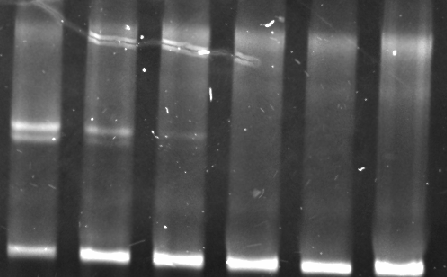
\includegraphics[width=\textwidth]{reconstnuc_a}
    \caption{Plain DNA}
    \label{fig:reconstnuc_a}
  \end{subfigure}
  \begin{subfigure}[htpb]{0.4\textwidth}
    \centering
    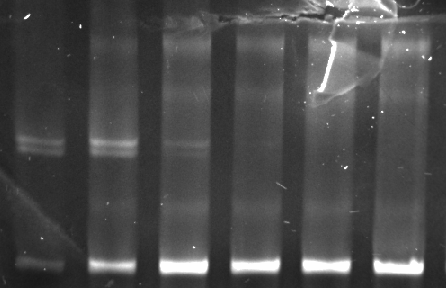
\includegraphics[width=\textwidth]{reconstnuc_b}
    \caption{Half-C-methylated DNA}
    \label{fig:reconstnuc_b}
  \end{subfigure}
  \begin{subfigure}[htpb]{0.4\textwidth}
    \centering
    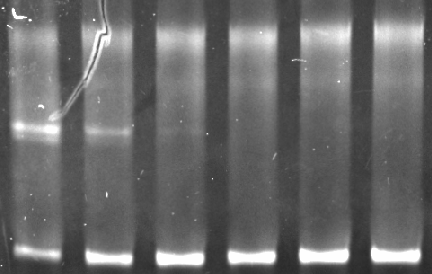
\includegraphics[width=\textwidth]{reconstnuc_c}
    \caption{All-C-methylated DNA}
    \label{fig:reconstnuc_c}
  \end{subfigure}
  \begin{subfigure}[htpb]{0.4\textwidth}
    \centering
    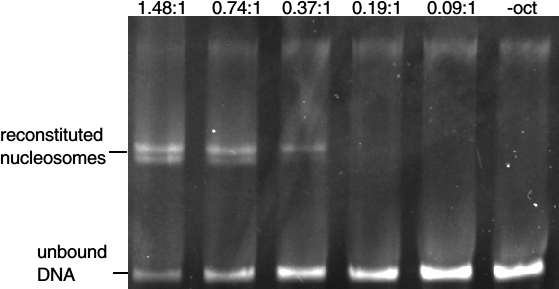
\includegraphics[width=\textwidth]{reconstnuc_d}
    \caption{CpG-methylated DNA}
    \label{fig:reconstnuc_d}
  \end{subfigure}
  \caption{First-cycle EMSA in 6\% DNA retardation gels for the four experimental groups.  Lanes for all images correspond to these histone:octamer ratios (left to right): (1) 1.48:1, (2) 0.74:1, (3) 0.37:1, (4) 0.19:1, (5) 0.09:1, and (6) DNA without histone octamer added.  These results are representative for all cycles.}
  \label{fig:reconstnuc}
\end{figure}

\subsection{Sequence preferences from fast Fourier transform analysis}
\label{ssec:nuseqpref_fft}

The frequency of each of the four nucleotides at each position along the reads was calculated (figure~\ref{fig:enriched_counts}). The frequency of each nucleotide showed periodicities of approximately 10 bp, as suggested by fast Fourier transform (figure~\ref{fig:enriched_power}).  The results also indicate that the synthetic library in enriched in G and T nucleotides.

\begin{figure}[htbp]
  \centering
  \begin{subfigure}[htbp]{0.8\textwidth}
    \centering
    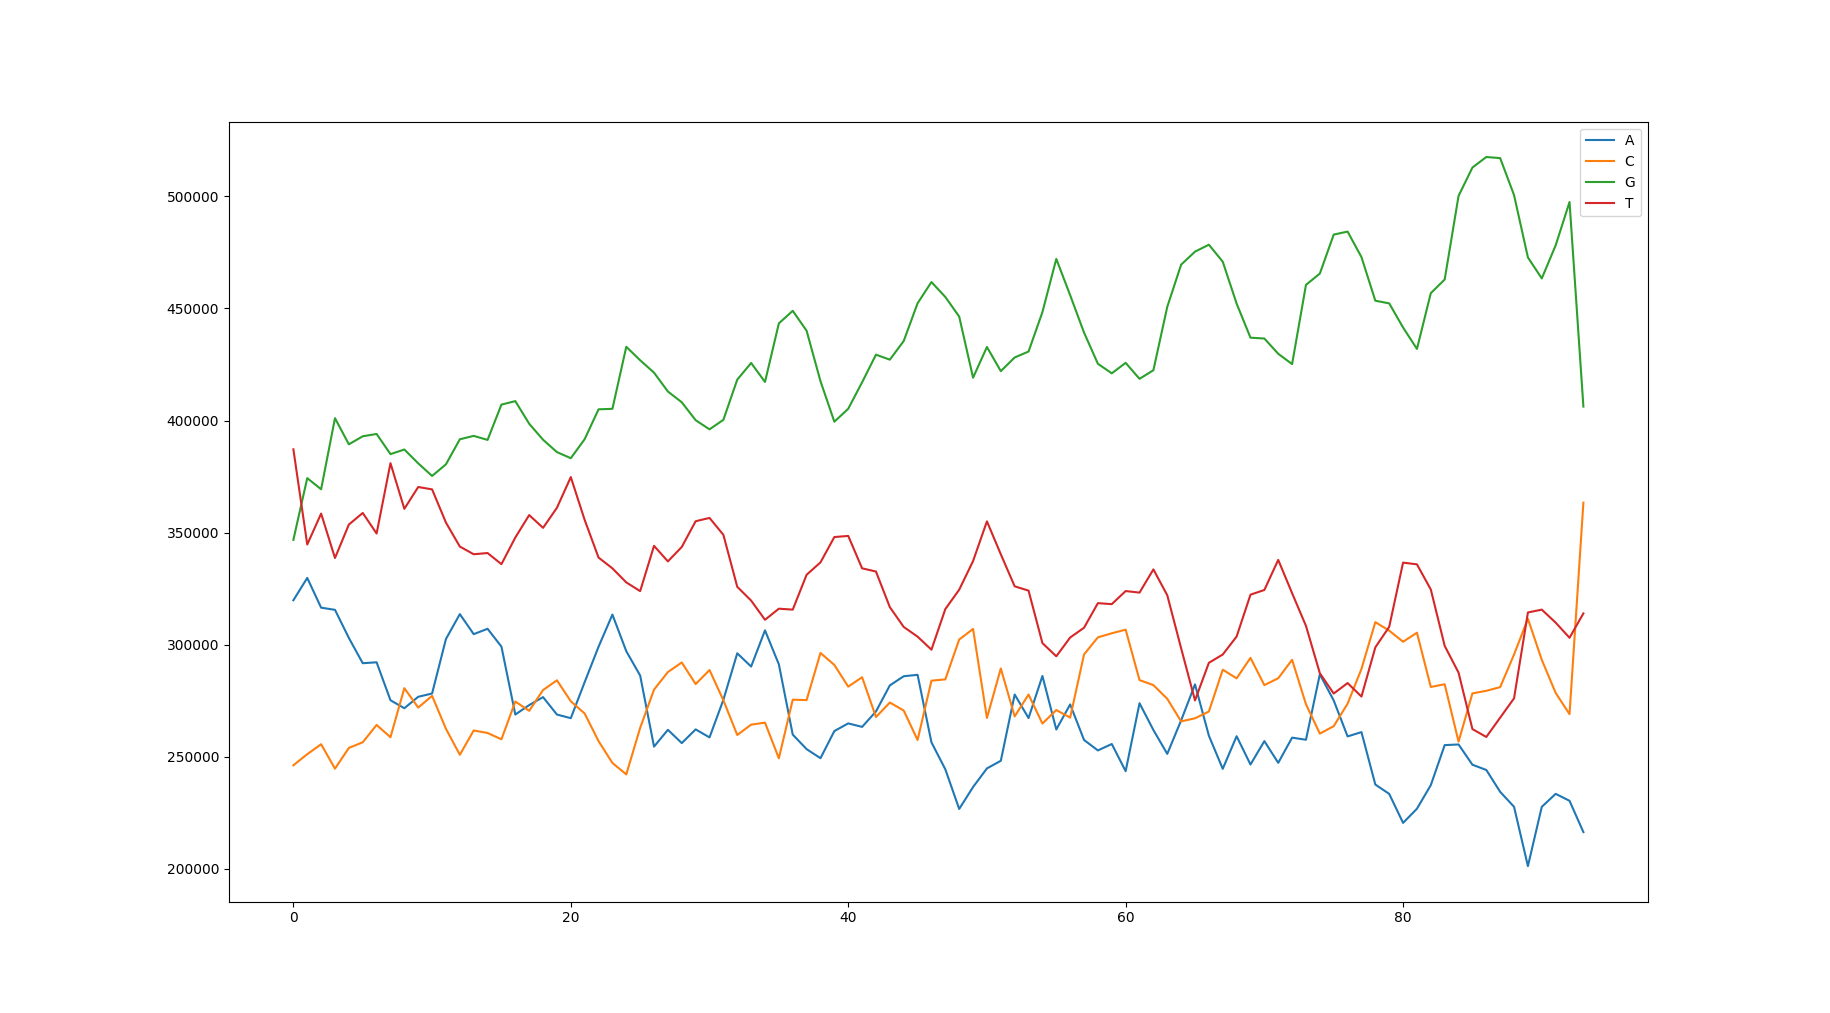
\includegraphics[width=0.8\textwidth]{enriched-counts}
    \caption{}
    \label{fig:enriched_counts}
  \end{subfigure}
  \begin{subfigure}[htbp]{0.8\textwidth}
    \centering
    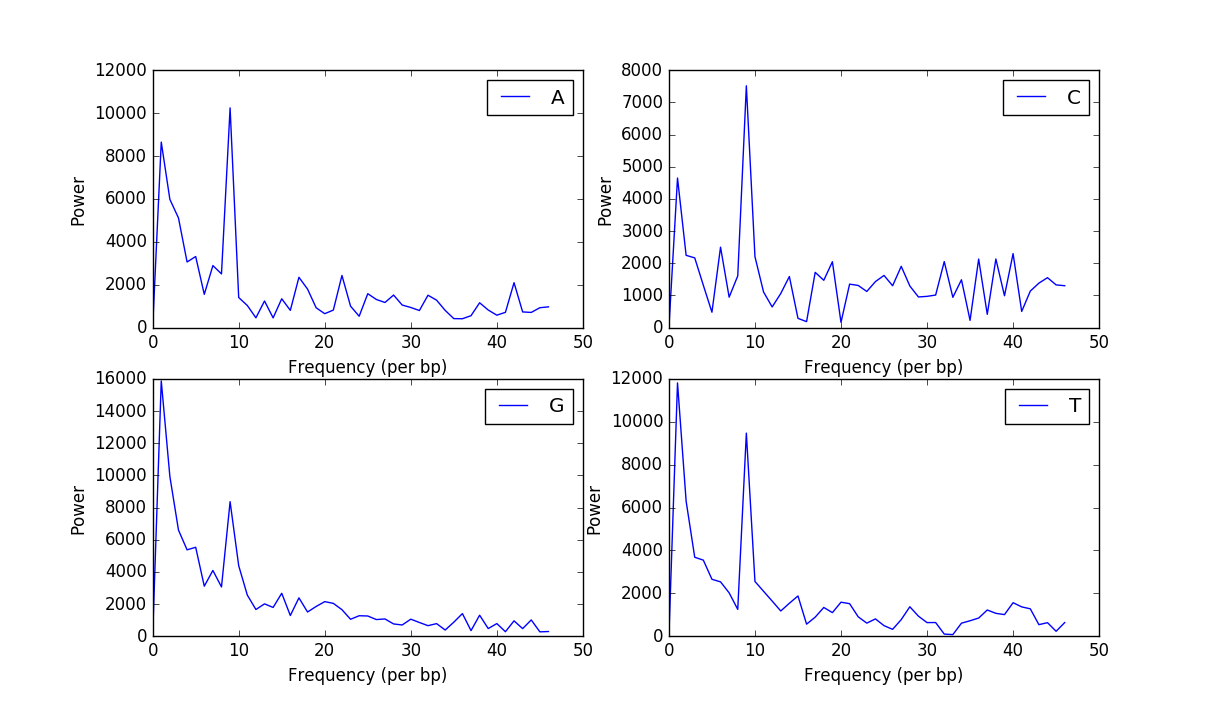
\includegraphics[width=0.8\textwidth]{enriched-power}
    \caption{}
    \label{fig:enriched_power}
  \end{subfigure}
  \caption{Analysis of a library of plain DNA bound to nucleosomes. (a) Nucleotide counts as a function of position along the reads; (b) Fast Fourier transform power spectra for the four nucleotides.}
  \label{fig:enriched}
\end{figure}

Similarly, we further examined the frequency of all dinucleotide sequences at each position along the reads in all libraries.  The data from the fourth cycle of nucleosome EMSA-SELEX were used in all subsequent analyses because they exhibited the strongest signals.  All bound DNA libraries showed a clear periodicity in mononucleotide and dinucleotide frequencies (figure~\ref{fig:freqplots}).  Specifically, half-C-methylated and all-C-methylated DNA showed the strongest signals, CpG-methylated DNA showed signals of intermediate strength, and plain DNA showed the weakest signals.  Fast Fourier transform confirmed that this periodicity was at approximately 0.1 per base pair (figure~\ref{fig:powerspectra_bound}).  Among the octamer:DNA ratios tested, the 1:0.74 ratio gave the strongest signals, and the signal intensity decreased as the proportion of histone octamer decreased (data not shown).  Libraries corresponding to this octamer:DNA ratio were therefore used for all subsequent analyses.

In contrast, all unbound DNA libraries were depleted of the periodic signal (figure~\ref{fig:powerspectra_unbound}).

\begin{figure}[htbp]
  \centering
  \begin{subfigure}[htbp]{0.6\textwidth}
    \centering
    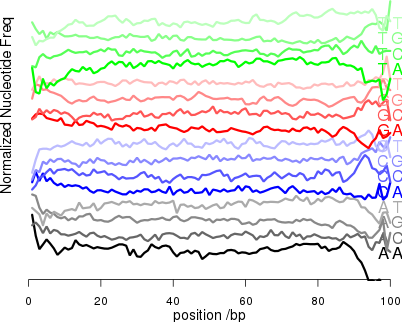
\includegraphics[width=0.6\textwidth]{emsa_e8_counts}
    \caption{Plain DNA}
    \label{fig:freqplots_e8}
  \end{subfigure}
  \begin{subfigure}[htbp]{0.6\textwidth}
    \centering
    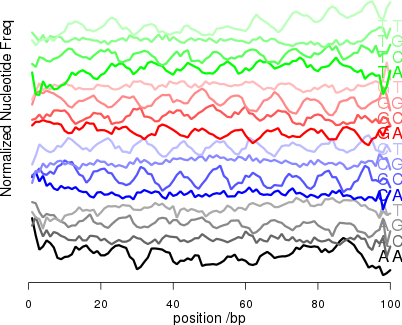
\includegraphics[width=0.6\textwidth]{emsa_f8_counts}
    \caption{Half-C-methylated}
    \label{fig:freqplots_f8}
  \end{subfigure}
  \begin{subfigure}[htbp]{0.6\textwidth}
    \centering
    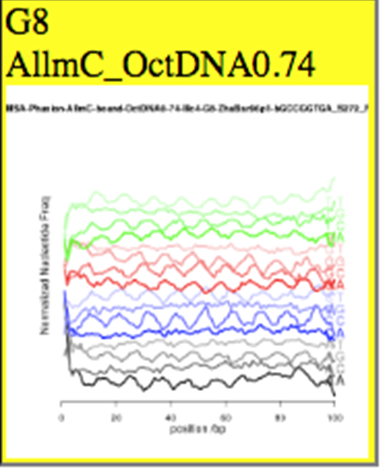
\includegraphics[width=0.6\textwidth]{emsa_g8_counts}
    \caption{All-C-methylated}
    \label{fig:freqplots_g8}
  \end{subfigure}
  \begin{subfigure}[htbp]{0.6\textwidth}
    \centering
    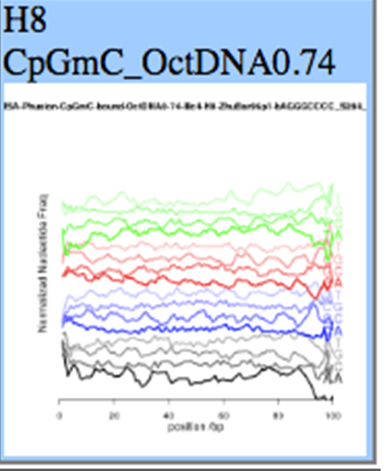
\includegraphics[width=0.6\textwidth]{emsa_h8_counts}
    \caption{CpG methylated}
    \label{fig:freqplots_h8}
  \end{subfigure}
  \caption{Frequencies of each mononucleotide and dinucleotide along the sequencing reads from libraries corresponding to 1:0.74 octamer:DNA ratios for the fourth cycle of EMSA-SELEX}
  \label{fig:freqplots}
\end{figure}

\begin{figure}[htbp]
  \centering
  \begin{subfigure}[htbp]{0.6\textwidth}
    \centering
    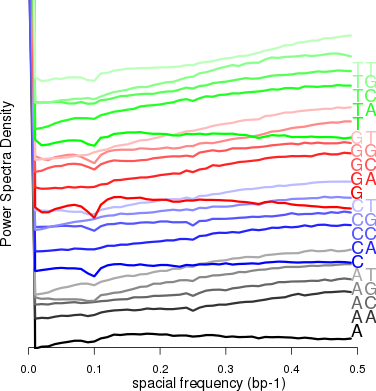
\includegraphics[width=0.6\textwidth]{emsa_g7_power}
    \caption{DNA not bound to nucleosomes}
    \label{fig:powerspectra_unbound}
  \end{subfigure}
  \begin{subfigure}[htbp]{0.6\textwidth}
    \centering
    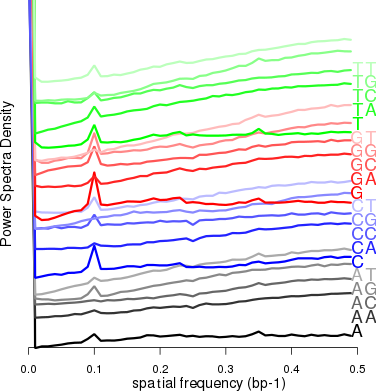
\includegraphics[width=0.6\textwidth]{emsa_g8_power}
    \caption{DNA bound to nucleosomes, 1:074 octamer:DNA}
    \label{fig:powerspectra_bound}
  \end{subfigure}
  \caption{Power spectra showing the effect of nucleosome binding on sequence periodicity.  Libraries from the all-C-methylated group in the fourth cycle of nucleosome EMSA-SELEX were shown here as representative spectra.  Other experimental groups showed similar patterns.}
  \label{fig:powerspectra}
\end{figure}

The phases and the amplitudes resulting from the fast Fourier transforms were then characterised, based on a periodicity of 10.2 bp (figure~\ref{fig:radial_mc}).

In all experimental groups, AA occurred at a phase of approximately \ang{300}.  TA occurred approximately out of phase with GC, but this is less pronounced in the plain DNA group compared to the methylated DNA groups.

When the cytosines were methylated, the amplitude for dinucleotides beginning with C increased, and their phases became more aligned.  In the plain DNA bound library, the CA, CC, TC, and CT sequences were spread out over phases of \ang{80} to \ang{180} (figure~\ref{fig:radial_mc_plain}).  In the half-C-methylated and all-C-methylated libraries for the same octamer:DNA ratio, these sequences were spread out over phases of \ang{70} to \ang{140} (figures~\ref{fig:radial_mc_halfmc} and~\ref{fig:radial_mc_allmc}).  These dinucleotides became more aligned to TC.  The phases of GA and GG also became more aligned.  Additionally, using the AA sequence as a reference, the amplitudes for CT and CA were greater in the all-C-methylated library than in the half-C-methylated library.  AA was used as a reference as its amplitude theoretically does not change. %citation needed.

These effects were less pronounced for CpG methylation (figure~\ref{fig:radial_mc_cpg}).  Relative to AA, the amplitudes of CC and CT increased.  However, the CA, CC, TC, and CT sequences were still spread over a wide range of phases, covering \ang{80} to \ang{160}.

\begin{figure}[htbp]
  \centering
  \begin{subfigure}[htbp]{0.6\textwidth}
    \centering
    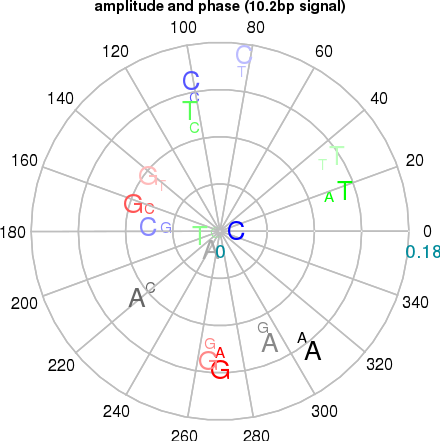
\includegraphics[width=0.6\textwidth]{emsa_e8_radial}
    \caption{Plain DNA}
    \label{fig:radial_mc_plain}
  \end{subfigure}
  \begin{subfigure}[htbp]{0.6\textwidth}
    \centering
    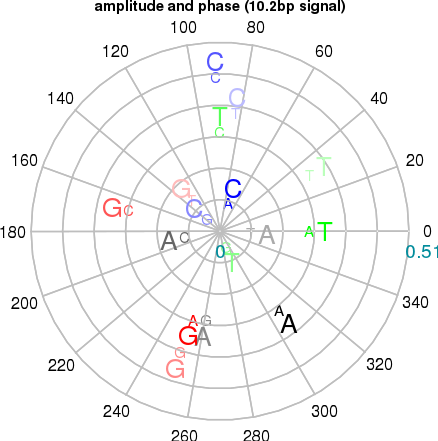
\includegraphics[width=0.6\textwidth]{emsa_f8_radial}
    \caption{Half-C-methylated}
    \label{fig:radial_mc_halfmc}
  \end{subfigure}
  \begin{subfigure}[htbp]{0.6\textwidth}
    \centering
    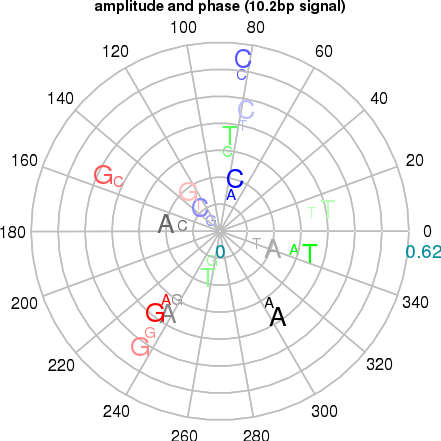
\includegraphics[width=0.6\textwidth]{emsa_g8_radial}
    \caption{All-C-methylated}
    \label{fig:radial_mc_allmc}
  \end{subfigure}
  \begin{subfigure}[htbp]{0.6\textwidth}
    \centering
    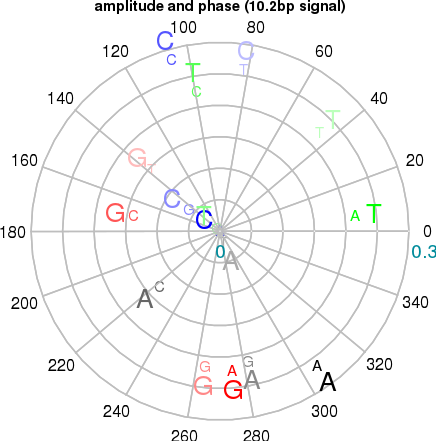
\includegraphics[width=0.6\textwidth]{emsa_h8_radial}
    \caption{CpG methylated}
    \label{fig:radial_mc_cpg}
  \end{subfigure}
  \caption{Radial plots showing the effect of cytosine methylation.  Angles indicate phases, and radii indicate amplitudes of dinucleotides based on a periodicity of 10.2 bp.}
  \label{fig:radial_mc}
\end{figure}

Certain dinucleotides containing cytosines were enriched when the cytosines were methylated, especially upon CpG methylation (figure~\ref{fig:c2nt}).  In particular CC, CG, and GC were enriched in the CpG methylated group.  In contrast, CC was depleted in the all-C-methylated group.  As the sequence preference is weak for nucleosomes, in all samples, the dinucleotide counts in the bound library relative to the dinucleotide counts in the corresponding unbound library did not deviate much from 1.0.

\begin{figure}[htbp]
  \centering
  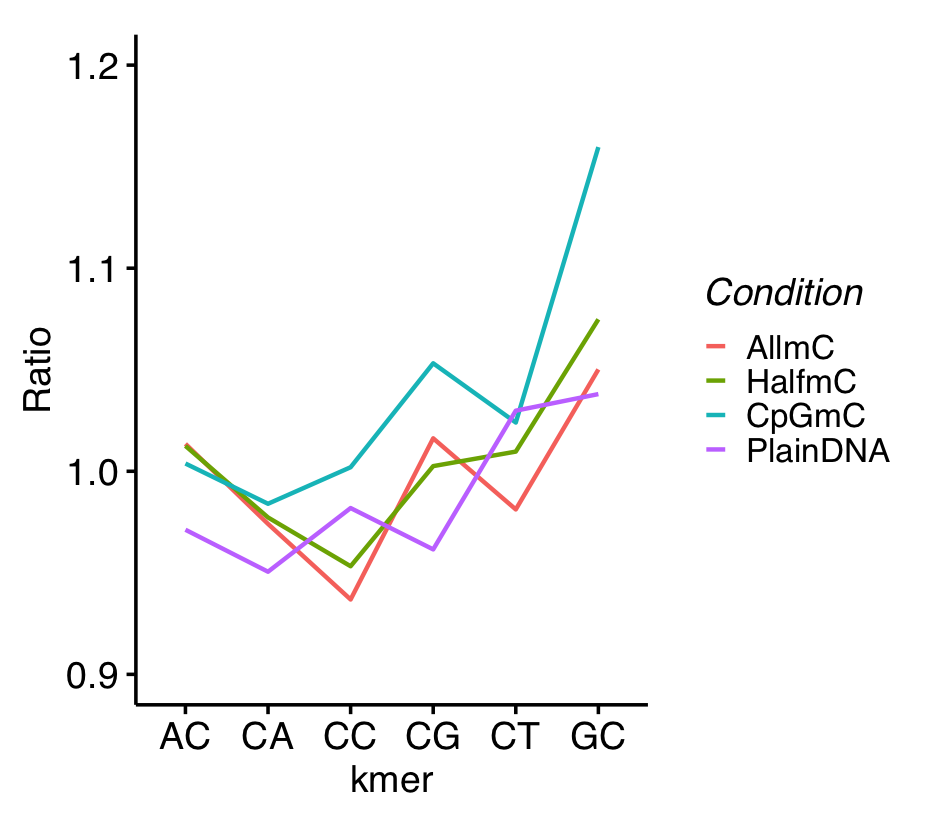
\includegraphics[width=0.6\textwidth]{c2nt}
  \caption{Enrichment of dinucleotides in the 0.74:1 octamer:DNA ratio libraries for each experimental group.  The number of occurrences of each dinucleotide in each library was calculated.  Dividing the count from the bound DNA library by the count from the unbound DNA library gave the ratios shown.} 
  \label{fig:c2nt}
\end{figure}

\subsection{Sequence preferences from sequence \emph{k}-mer counts}
\label{ssec:nuseqpref_kmer}

For each library, the number of occurrences of each possible continuous 9-mer of nucleotides was counted.

Low correlation between bound and unbound libraries for CpG-methylated and half-C-methylated groups were observed (figure~\ref{fig:kmer_bound_cpg} and figure~\ref{fig:kmer_bound_half}), suggesting that bound and unbound libraries have different enriched signals.  For these experimental groups, the unbound libraries exhibit at A/T-bias, as indicated by A-rich \emph{k}-mers and T-rich \emph{k}-mers being more represented in unbound libraries than the bound library for the same experimental group.  This effect was stronger for the CpG-methylated group.  In contrast, there was a relatively high positive correlation between bound and unbound libraries for the all-C-methylated group (figure~\ref{fig:kmer_bound_all}).  This suggested that the bound and unbound libraries are more similar, and that the effect of the nucleosome disfavouring A/T-rich sequences was weaker for all-C-methylated DNA.

However, both the bound and unbound all-C-methylated libraries -- relative to the corresponding bound or unbound plain DNA library -- exhibited the same direction of bias (figure~\ref{fig:kmer_bias}).  The same behaviour for both the bound and the unbound is likely explained by PCR bias, that is, methylated dCTP has a lower efficiency to be incorporated during PCR.  More specifically, the biases were stronger for the bound libraries.

\begin{figure}[htbp]
  \centering
  \begin{subfigure}[htbp]{0.8\textwidth}
    \centering
    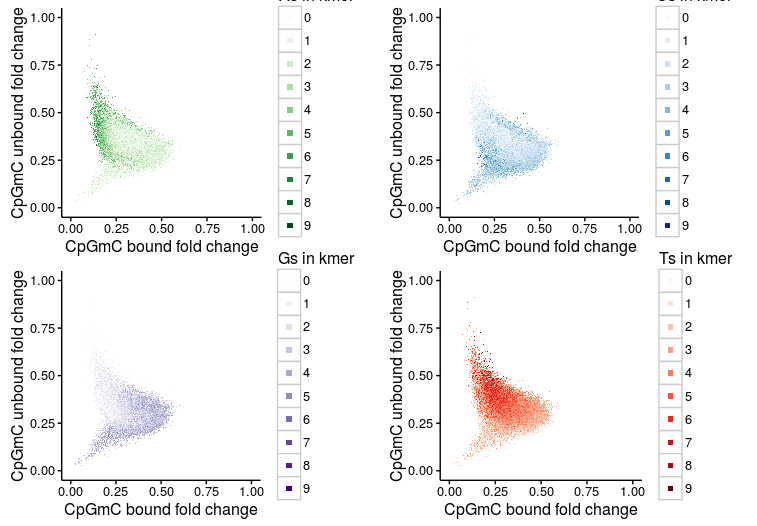
\includegraphics[width=0.8\textwidth]{kmer_CpGubXCpGb}
    \caption{CpG methylated, R = -0.402}
    \label{fig:kmer_bound_cpg}
  \end{subfigure}
  \begin{subfigure}[htbp]{0.8\textwidth}
    \centering
    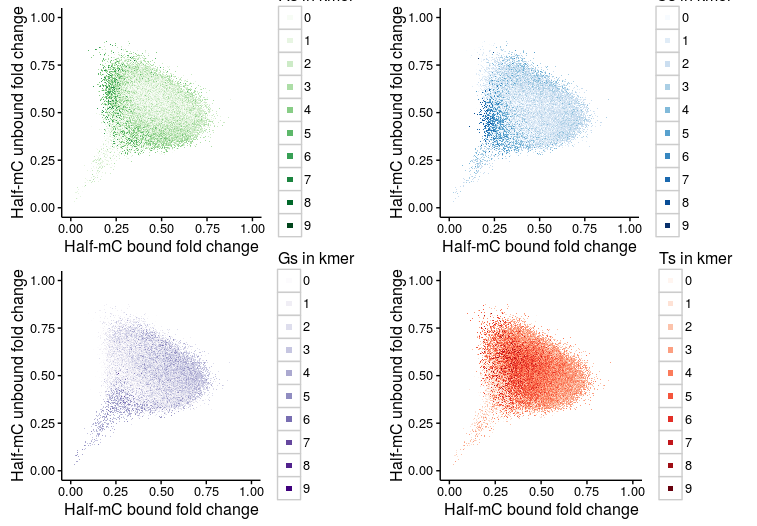
\includegraphics[width=0.8\textwidth]{kmer_halfubXhalfb}
    \caption{Half-C-methylated, R = -0.226}
    \label{fig:kmer_bound_half}
  \end{subfigure}
  \begin{subfigure}[htbp]{0.8\textwidth}
    \centering
    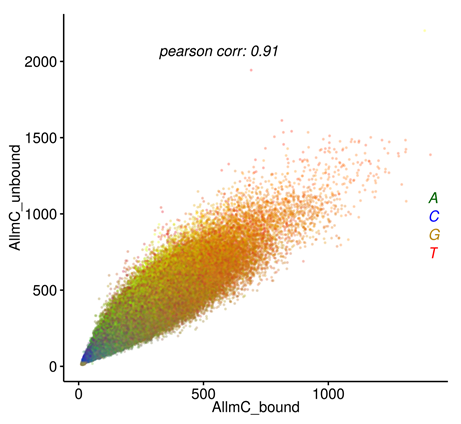
\includegraphics[width=0.8\textwidth]{kmer_allubXallb}
    \caption{All-C-methylated, R = +0.710}
    \label{fig:kmer_bound_all}
  \end{subfigure}
  \caption{9-mer count scatter plots showing the effect of nucleosome reconstitution on each experimental group.  Each point represents a nucleotide 9-mer and the shading (A: green, C: blue, G: purple, T: red) indicates the number of the respective nucleotide in the 9-mer.  9-mer counts were normalised against lig147 to give fold changes.}
  \label{fig:kmer_bound}
\end{figure}

\begin{figure}[htbp]
  \centering
  \begin{subfigure}[htbp]{0.8\textwidth}
    \centering
    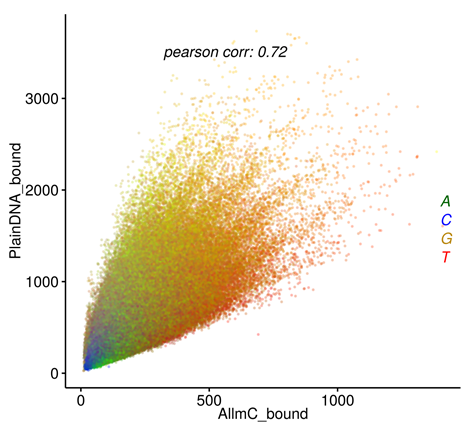
\includegraphics[width=0.8\textwidth]{kmer_plainbXallb}
    \caption{Bound DNA, R = -0.162}
    \label{fig:kmer_bias_bound}
  \end{subfigure}
  \begin{subfigure}[htbp]{0.8\textwidth}
    \centering
    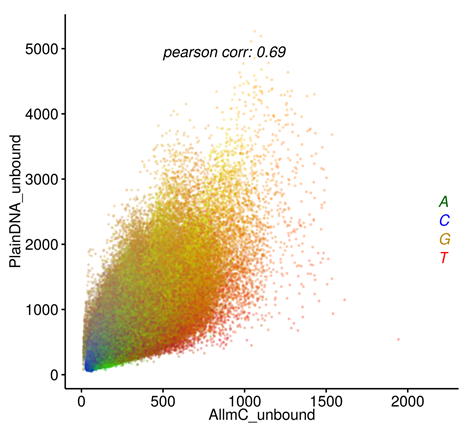
\includegraphics[width=0.8\textwidth]{kmer_plainubXallub}
    \caption{Unbound DNA, R = -0.479}
    \label{fig:kmer_bias_unbound}
  \end{subfigure}
  \caption{9-mer count scatter plots showing similar sequence biases in bound and unbound libraries.  Each point represents a nucleotide 9-mer and the shading (A: green, C: blue, G: purple, T: red) indicates the number of the respective nucleotide in the 9-mer.  9-mer counts were normalised against lig147 to give fold changes.}
  \label{fig:kmer_bias}
\end{figure}

The frequencies of continuous stretches of adenines (A-stretches) were also counted in each library (figure~\ref{fig:astretch}).  Methylation was associated with A-stretches being depleted in the libraries containing DNA bound to nucleosomes.  Compared to plain DNA, the half-C-methylated and all-C-methylated groups exhibited greater depletions in A-stretches.  This effect was more pronounced in the CpG methylated group.  Almost all of the groups exhibited ratios below 1.0.  This suggests that A-stretches are disfavoured in nucleosome binding, and this disfavouring is likely enhanced when cytosines are methylated.

\begin{figure}[htbp]
  \centering
  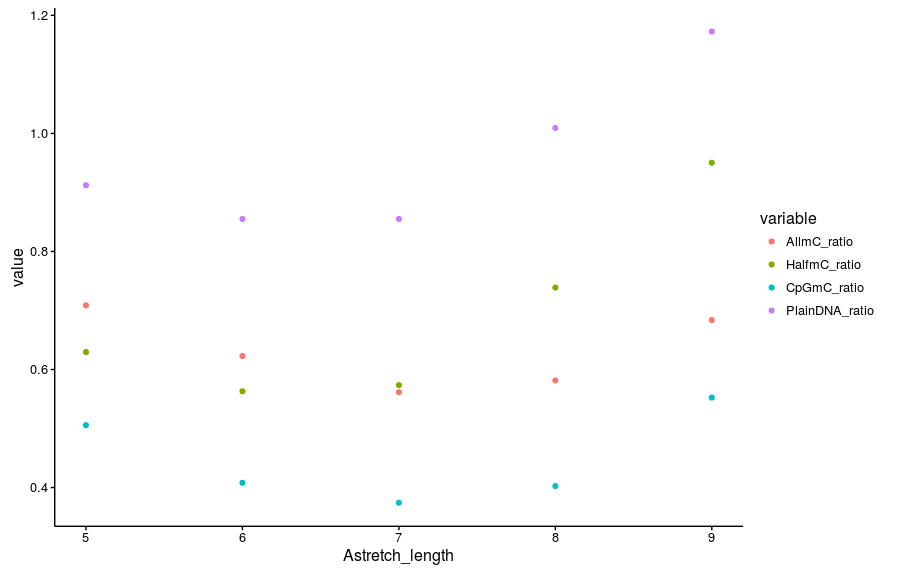
\includegraphics[width=0.6\textwidth]{astretch}
  \caption{Enrichment of continuous stretches of adenines for each experimental group.  The number of occurrences of each adenine \emph{k}-mer in each library was calculated (e.g. `5' corresponds to `AAAAA').  Dividing the count from the bound DNA library by the count from the unbound DNA library gave the ratios shown.}
  \label{fig:astretch}
\end{figure}

\section{Discussion}
\label{sec:emsaselex_discussion}

\subsection{Mechanisms leading to nucleosome sequence preferences}
\label{ssec:emsaselex_discussion_seqpref}

From nucleosome EMSA-SELEX, nucleosome binding introduced an approximately 10-bp periodicity in mononucleotide and dinucleotide frequencies.  These observations confirmed previous studies that suggest a $\sim$10-bp helical repeat in DNA within chromatin and that dinucleotides that confer flexibility are positioned at the same phase of the periodicity \citep{struhl_determinants_2013}.  Furthermore, phases and amplitudes of the dinucleotides supported findings that indicate that TA occurs out of phase with GC \citep{struhl_determinants_2013}.  This preference is confirmed in our experiment.

Stretches of adenines between five and nine nucleotides were depleted in libraries of DNA bound to nucleosomes, as indicated by normalised counts below 1.0 (figure~\ref{fig:astretch}).  Previous experiments with plain DNA libraries enriched for signal by the group suggested that A-stretches were depleted as their length increases.  These agree with studies that reveal that poly(dA) tracts disfavour nucleosome positioning because they make DNA stiff and therefore not conducive to the bending needed for nucleosome positioning \citep{struhl_determinants_2013}.  Trends suggested that A-stretches were more depleted in methylated DNA than in plain DNA.  However, the signals from plain DNA were weak and the significance of these depletions cannot be assessed with the one biological replicate used in the experiment.  To draw better conclusions, additional replicates should be performed.

In sum, nucleosome EMSA SELEX with current deep sequencing methods were able to reveal sequence preferences for nucleosomes.  These sequence preferences are similar to that from MNase-based assays in previous research.  Additionally, as this is the first time nucleosome EMSA-SELEX was performed with methylated cytosines, results therefore suggest that this technique can be adapted to reconstitute nucleosomes containing methylated DNA.

\subsection{Effect of methylation on nucleosome sequence preferences}
\label{ssec:emsaselex_discussion_methyl}

When cytosine were methylated in CpG methylation and CH methylation contexts, the amplitude of the 10 bp periodicity of sequences became stronger.  This means that biases towards sequences conducive to nucleosome binding were stronger, and this may be explained by how methylated cytosines in CpG methylation disfavours nucleosome positioning \citep{huff_dnmt1-independent_2014, ,kelly_genome-wide_2012}.

Additionally, when cytosines were methylated, the amplitudes of CC, GG, and GC dinucleotides increased, and the phases of CC, CT, TC, and CA lined up more.  Methylation of cytosines makes DNA more rigid \citep{rao_systematic_2018, perez_impact_2012}.  Therefore, a possible explanation of this observation is that as more cytosines are methylated, rigid sequences are more strongly associated with phase angles that do not interfere with the bendability of DNA in such a way that would interfere with nucleosome positioning.  Another explanation is that methylated cytosines are structurally similar to thymines -- bulkier -- and therefore behaves more like thymines.  This explains TC and CC having similar phases, but does not explain why TT does not share this similarity.  Further molecular simulation studies would be required to elucidate the structural basis of the observations.

Cytosine methylation was also observed to be associated with enrichment of certain dinucleotides containing cytosines (figure~\ref{fig:c2nt}), but the effect size is small.  Small deviations from 1:1 ratios can be attributed to the low selectivity of histone octamers to DNA, as compared to transcription factors \citep{struhl_determinants_2013}. % probably find better citation to support this assertion, admittedly the sentence i was thinking of is not that strong
However, additional biological replicates must be done in order to evaluate the significance of the deviations from 1:1 ratios for each dinucleotide exhibited by each experimental group.

Investigating nucleotide 9-mers suggests that for CpG-methylated DNA and half-C-methylated DNA, the nucleosomes disfavoured A/T-rich 9-mers.  This nucleosome preference against A/T-rich sequences is similar to how unmethylated DNA disfavours tracts of adenines and thymines \citep{struhl_determinants_2013}. However, this bias was less apparent in half-C-methylated DNA than in CpG-methylated DNA, and disappeared from all-C-methylated DNA (figure~\ref{fig:kmer_bound_all}).

Thus these results provide preliminary insights into \emph{in vitro} sequence preferences for nucleosomes binding to CpG-methylated and CH-methylated DNA.  Further study could lead to better insights on how organisms use both forms of methylation to position nucleosomes, control transcription, and in turn regulate developmental and physiological processes.

Calculating sequence enrichments in the all-C-methylated group relative to the plain DNA group revealed that similar biases were present in both unbound and bound DNA.  Most likely, PCR bias accounted for the similar biases exhibited by both bound and unbound DNA.  Quantifying the sequence biases introduced by PCR would then allow removal of this bias to reveal the biases introduced by nucleosome sequence preferences.

\section{Materials and Methods}
\label{sec:emsaselex_methods}

\subsection{DNA ligand design and preparation}
\label{ssec:emsaselex_methods_lig}

The sequence of the initial input library (lig147) is \texttt{5' GCTCTTCCGATCT nnnnnnnnn\-nnnnnnnnnnn AGATCGGAAGAGC 3'}, where n denotes any nucleotide chosen at random. The input library DNA was made up to \SI{200}{\nano\Molar} in TE buffer with \SI{0.2}{\milli\Molar} EDTA at pH 8.0.

PCR amplification was adapted from manufacturer's recommended protocols for Phusion High-Fidelity DNA Polymerase (ThermoFisher, F530).  The sequence of the forward primer was \texttt{5' CCCTACACGAC GCTCTTCC 3'}, and the sequence of the reverse primer was \texttt{5' CAGACGTGT GCTCTTCCG 3'}.  Thirteen cycles of PCR with recommended temperatures were followed by ten cycles with the \SI{98}{\celsius} denaturation temperature replaced with \SI{72}{\celsius}.  For the `half-C-methylated group', half of the dCTPs in the amplification mix were replaced with 5-methyl dCTP, and for the `all-C-methylated group', all of the dCTPs were replaced with 5-methyl dCTP.  To create the libraries for the CpG-methylated group, plain DNA was incubated with methyltransferase (M.SssI), S-adenomethionine, and \ce{MgCl2} according to the protocols suggested by the enzyme manufacturer.

\subsection{Nucleosome EMSA-SELEX}
\label{ssec:emsaselex_methods_selex}

Nucleosomes were reconstituted from DNA libraries and \emph{Xenopus laevis} histone octamers using \SI{2}{\Molar} \ce{KCl} refolding buffer and periodic addition of dilution buffer as described by \citet{dyer_reconstitution_2003} (`Reconstitution of Nucleosome Core Particles').  Reconstituted nucleosomes were analysed by EMSA(electrophoretic mobility shift assay) by using TBE 6\% DNA retardation gel and 0.2\% TBE buffer on ice.  For the 1.48:1 octamer:DNA ratio, the faster-migrating gel band corresponding to DNA not bound to nucleosomes was silced.  The slower-migrating bands corresponding to DNA bound to nucleosomes were sliced for all other octamer:DNA ratios.  The sliced bands were dissolved in \SI{70}{\micro\litre} Tris pH 8.0, and then incubated at \SI{70}{\celsius} overnight to elute DNA.  Eluted DNA was amplified using procedures adapted from manufacturer's recommended protocols for Phusion High-Fidelity DNA Polymerase.  Here, 21 cycles of PCR with a \SI{98}{\celsius} denaturation temperature and a \SI{67}{\celsius} annealing temperature were followed by 10 cycles with a \SI{79}{\celsius} denaturation temperature and a \SI{64}{\celsius} annealing temperature.  Four such rounds of nucleosome EMSA-SELEX were carried out.

\subsection{Sequencing}
\label{ssec:emsaselex_methods_seq}

The eluted DNA was barcoded for sequencing.  Amplification was carried out using the procedures recommended for Phusion DNA polymerase for 29 PCR cycles, using \SI{5}{\micro\Molar} barcoded PE primer obtained from IDT.  All barcoded DNA was then pooled together and purified using 1.2x AMPure beads once (Beckman Coulter) according to manufacturer's protocols.  Subsequently, the DNA was diluted to \SI{2}{\nano\Molar}.  Sequencing was performed using Illumina HiSeq 4000, following standard protocols, with $>$ 60 bp paired-end settings.  Raw sequences were demultiplexed, then the R1 and R2 reads of paired-end sequencing were merged according to \citet{zhu_interaction_2018}.

\subsection{Data analysis}
\label{ssec:emsaselex_methods_anal}

Fast Fourier transformation (FFT) was performed using the position along the read as the time domain and the frequency of mononucleotides or dinucleotides at a specific position within the read as the frequency domain, following \citet{zhu_interaction_2018}.  From this, power spectra for mononucleotides and dinucleotides were obtained.  The phases and amplitudes of FFT were also examined at a periodicity of 10.2 bp.

\chapter{PCR Bias}
\label{ch:pcrbias}

\section{Introduction}
\label{sec:pcrbias_intro}

\subsection{Origin of PCR bias}
\label{ssec:pcrbias_intro_origin}

PCR is a known source of bias in massively parallel sequencing \citep{olova_comparison_2018}.  Among the processes in Illumina sequencing, PCR amplification during library preparation has been identified as the major source of bias.  \citet{aird_analyzing_2011} measured frequencies of amplicons of varying GC content after each step in library preparation for Illumina sequencing, and found that DNA shearing, adapter ligation, gel size selection did not significantly introduce biases in response to GC content.  However, PCR depleted loci with GC content exceeding 65\% to the order of 1\% of the reference loci with intermediate GC content, and it also depleted loci with GC content lower than 12\% to the order of 10\% of the reference loci.  This pattern was observed even for 10 PCR cycles.

There are methods to mitigate this bias, including choosing the source for the DNA polymerase enzyme.  Phusion DNA polymerase is commonly used because it has higher processivity and fidelity than most polymerases \citep{quail_optimal_2012}.  \citet{aird_analyzing_2011} also showed that replacing Phusion with AccuPrime Taq HiFi polymerase improved PCR bias.  Extension at \SI{60}{\celsius} using this enzyme retained more low-GC sequences, but also led to a decrease in yield of GC-rich reads.  \citet{quail_optimal_2012} showed that replacing Phusion with Kapa HiFi led to a more uniform genome coverage.  However, this also led to a higher error rate, especially in TA-rich regions that Phusion often fails to amplify.

\subsection{How PCR bias affects reliability of sequencing results}
\label{ssec:pcrbias_intro_effects}

Commonly-used model organisms have GC content within the range in which bias is least likely introduced.  \emph{E. coli} and humans have genomes that have moderate GC content, with \emph{E. coli} having a GC content of 51\%.  However, PCR bias is still significant for these model organisms as they have important sequences that may be affected by PCR bias.  This includes single-nucleotide polymorphisms and GC-rich sequences like transcription start sites and first exons in eukaryotes.  %Additionally, humans exhibit `bad promoters'. % expand on the `bad promoters' data set from Ross et al.  Where did they get them, and what is their importance?

\subsection{Purpose of this study}
\label{ssec:pcrbias_intro_why}

Although it is well-characterised that PCR introduces sequence biases, it is unknown which process within procedures that employ PCR amplification contributes the most to this bias, and to which degree.  Specifically, the biases introduced from the number of PCR cycles, template concentrations, and from purification have not been characterised.  Such characterisation would be beneficial in developing a model to quantify PCR bias.  With such a model, these PCR biases can be removed in genomic studies to reveal true signals introduced by the factors tested in the relevant experiments.  PCR bias is also especially relevant for the first part of this study -- nucleosome EMSA-SELEX -- because sequence selectivity for the nucleosome is much weaker than transcription factors \citep{struhl_determinants_2013}.  This makes the signal enrichment in the sequencing library weak, and makes it difficult to separate signals introduced by nucleosome binding from biases introduced by PCR.  In other words, a large part of sequences preferences found in the libraries bound or unbound to nucleosomes can come from the PCR-introduced bias.

Here I assessed the sequence biases that could be introduced to the initial input library and during library amplifications for nucleosome EMSA-SELEX.  I tested sequence biases introduced by the choice of DNA polymerase, bottleneck effects, choice of reagent vendors, cycles of PCR, and purification of DNA after PCR.  From the resulting sequencing data, the distribution of \emph{k}-mer nucleotides was assessed.

\section{Results}
\label{sec:pcrbias_results}

The initial input library lig147 was amplified and processed, with conditions varied to test biases introduced by polymerase enzymes, DNA purification, and reagent vendors.  After the PCR products were sequenced, the frequencies of each possible continuous 9-mer of nucleotides was counted.

\subsection{Biases from DNA polymerase enzymes}
\label{ssec:pcrbias_result_enz}

Libraries amplified by Phusion, Phire, DreamTaq, and Q5 DNA polymerase enzymes were analysed.  For each enzyme, the library from 24 cycles of PCR was compared to the library from 8 cycles of PCR (figure~\ref{fig:kmer_enz}).  High correlation coefficients between 8-cycle libraries and 24-cycle libraries for all enzymes sources were observed, suggesting that libraries were similar within each pair.  Thus, the effect from PCR is moderate for about 15 cycles of PCR amplification.  All enzymes showed slight biases towards A and T, with Phusion exhibiting the weakest bias and Phire exhibiting the strongest bias.

\begin{figure}[htbp]
  \centering
  \begin{subfigure}[htbp]{0.6\textwidth}
    \centering
    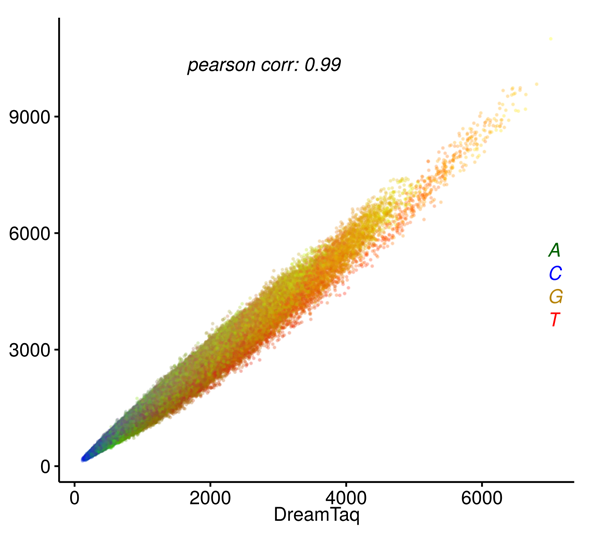
\includegraphics[width=0.6\textwidth]{kmer_dreamtaq}
    \caption{DreamTaq, R = 0.709}
    \label{fig:kmer_enz_dreamtaq}
  \end{subfigure}
  \begin{subfigure}[htbp]{0.6\textwidth}
    \centering
    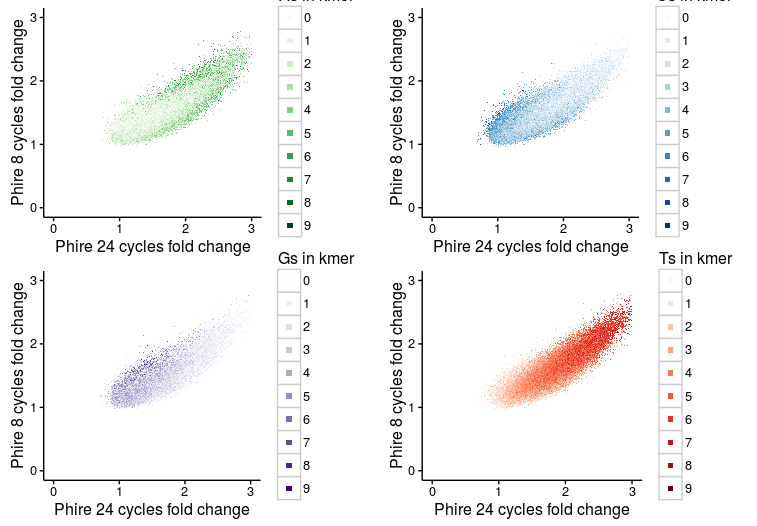
\includegraphics[width=0.6\textwidth]{kmer_phire}
    \caption{Phire, R = 0.839}
    \label{fig:kmer_enz_phire}
  \end{subfigure}
  \begin{subfigure}[htbp]{0.6\textwidth}
    \centering
    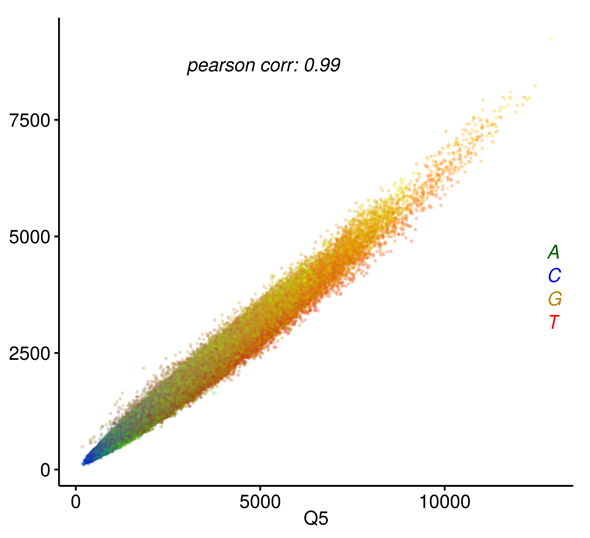
\includegraphics[width=0.6\textwidth]{kmer_q5}
    \caption{Q5, R = 0.760}
    \label{fig:kmer_enz_q5}
  \end{subfigure}
  \begin{subfigure}[htbp]{0.6\textwidth}
    \centering
    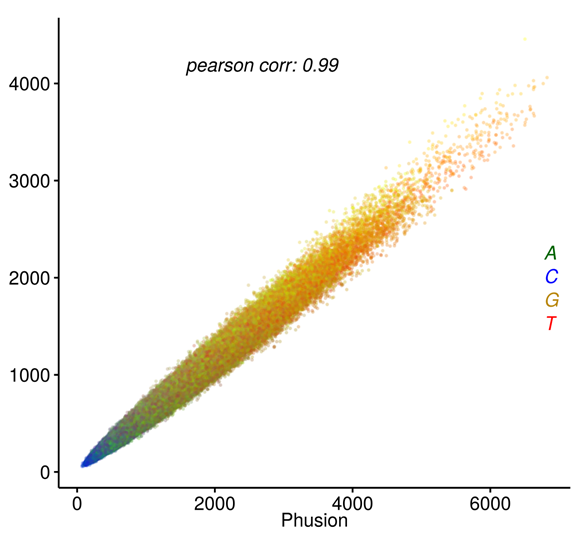
\includegraphics[width=0.6\textwidth]{kmer_phusion}
    \caption{Phusion, R = 0.659}
    \label{fig:kmer_enz_phusion}
  \end{subfigure}
  \caption{9-mer count scatter plots comparing biases from different polymerase enzymes.  Each point represents a nucleotide 9-mer and the shading (A: green, C: blue, G: purple, T: red) indicates the number of the respective nucleotide in the 9-mer.  9-mer counts were normalised against lig147 to give fold changes.}
  \label{fig:kmer_enz}
\end{figure}

\subsection{Biases from bottleneck effect}
\label{ssec:pcrbias_result_bn}

In SELEX, as limited DNA is bound by the target protein, a bottlenecking effect is applied between cycles.  This bottleneck effect on PCR bias was then investigated.  In this context, the bottleneck effect refers to how some members of a large DNA library are likely to be lost by chance if a small sample of the library is taken for amplification.  For each enzyme investigated in subsection~\ref{ssec:pcrbias_result_enz}, the PCR product after 24 cycles was diluted and $\frac{1}{2^{20}}$ of the samples from this dilution were used as template and amplified.  Comparing two samples for each enzyme suggested that bottleneck effects did not introduce large biases, as indicated by the strong correlations between the two samples for each enzyme (figure~\ref{fig:kmer_bn}).  However, Phire exhibited the greatest bias from the bottleneck effect, as revealed by the smallest correlation coefficient.

\begin{figure}[htbp]
  \centering
  \begin{subfigure}[htbp]{0.6\textwidth}
    \centering
    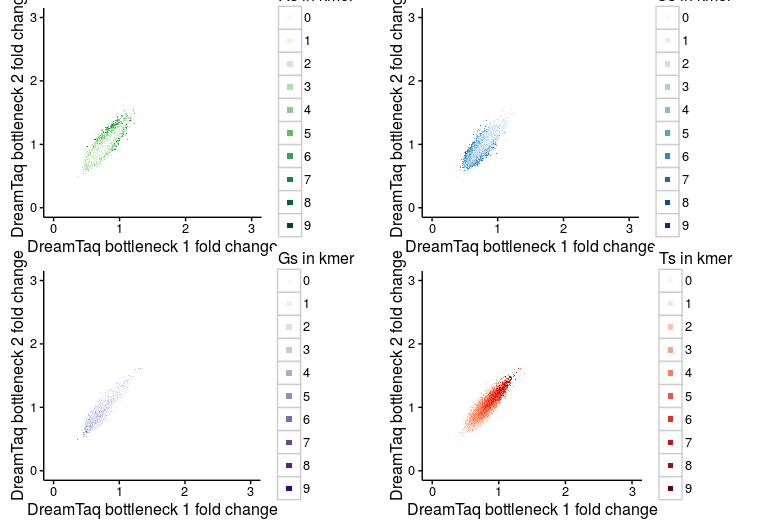
\includegraphics[width=0.6\textwidth]{kmer_dreamtaqBN}
    \caption{DreamTaq, R = 0.884}
    \label{fig:kmer_bn_dreamtaq}
  \end{subfigure}
  \begin{subfigure}[htbp]{0.6\textwidth}
    \centering
    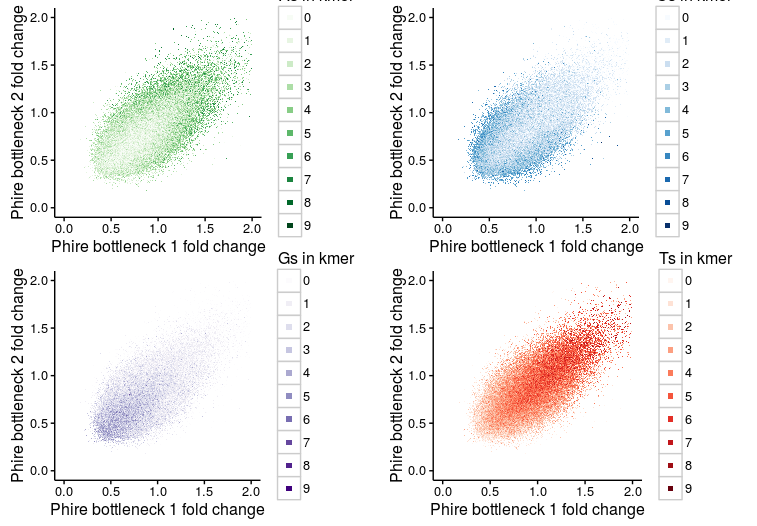
\includegraphics[width=0.6\textwidth]{kmer_phireBN}
    \caption{Phire, R = 0.697}
    \label{fig:kmer_bn_phire}
  \end{subfigure}
  \begin{subfigure}[htbp]{0.6\textwidth}
    \centering
    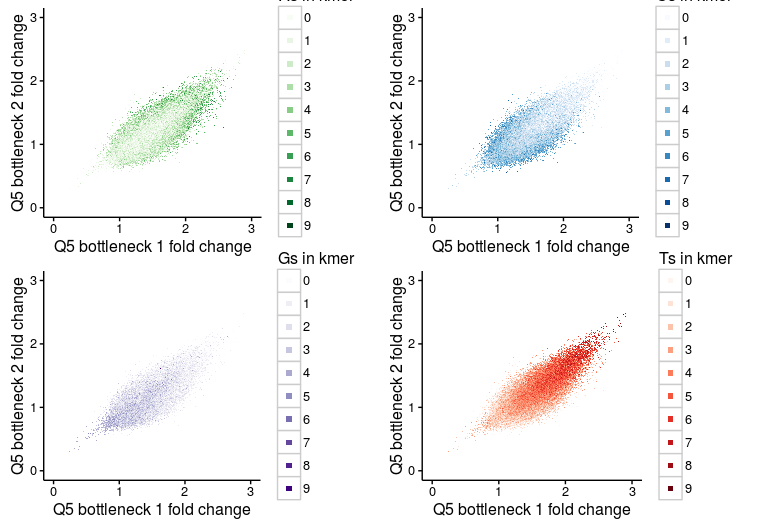
\includegraphics[width=0.6\textwidth]{kmer_q5BN}
    \caption{Q5, R = 0.767}
    \label{fig:kmer_bn_q5}
  \end{subfigure}
  \begin{subfigure}[htbp]{0.6\textwidth}
    \centering
    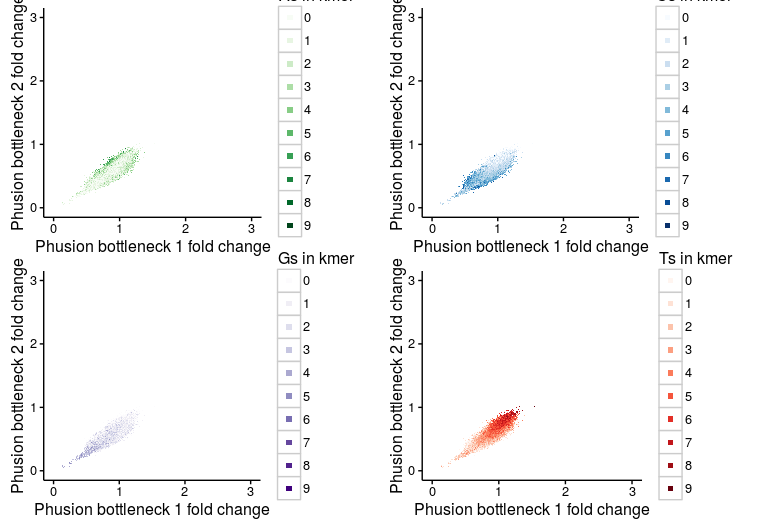
\includegraphics[width=0.6\textwidth]{kmer_phusionBN}
    \caption{Phusion, R = 0.844}
    \label{fig:kmer_bn_phusion}
  \end{subfigure}
  \caption{9-mer count scatter plots showing the bottleneck effect for different polymerase enzymes.  Each point represents a nucleotide 9-mer and the shading (A: green, C: blue, G: purple, T: red) indicates the number of the respective nucleotide in the 9-mer.  9-mer counts were normalised against lig147 to give fold changes.}
  \label{fig:kmer_bn}
\end{figure}

\subsection{Biases from purification}
\label{ssec:pcrbias_result_pur}

To investigate the effect of DNA purification, the lig147 input library was purified by AMPure beads for multiple times before sequencing.  The normalised 9-mer counts from the library after eight rounds of purification strongly correlated with that from the library after one round of purification (figure~\ref{fig:kmer_pur}).  This suggested that purification did not introduce strong nucleotide biases.

\begin{figure}[htbp]
  \centering
  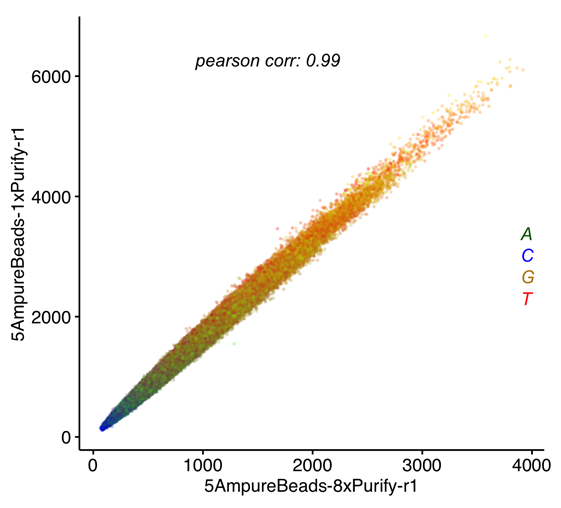
\includegraphics[width=0.8\textwidth]{kmer_ampure}
  \caption{9-mer count scatter plot showing the effect of AMPure bead purification.  Each point represents a nucleotide 9-mer and the shading (A: green, C: blue, G: purple, T: red) indicates the number of the respective nucleotide in the 9-mer.  9-mer counts were normalised against lig147 to give fold changes.  R = 0.865}
  \label{fig:kmer_pur}
\end{figure}

\subsection{Biases from reagent vendors}
\label{ssec:pcrbias_result_reagent}

Different combinations of four vendors for dNTPs -- including one source with dCTP replaced by 5-methyl dCTP -- and two vendors of Phusion High-Fidelity DNA polymerase were investigated.  The fractions of each nucleotide after 24 rounds of PCR were calculated for each combination (figure~\ref{fig:linearmodel_nt}).

\begin{figure}[htbp]
  \centering
  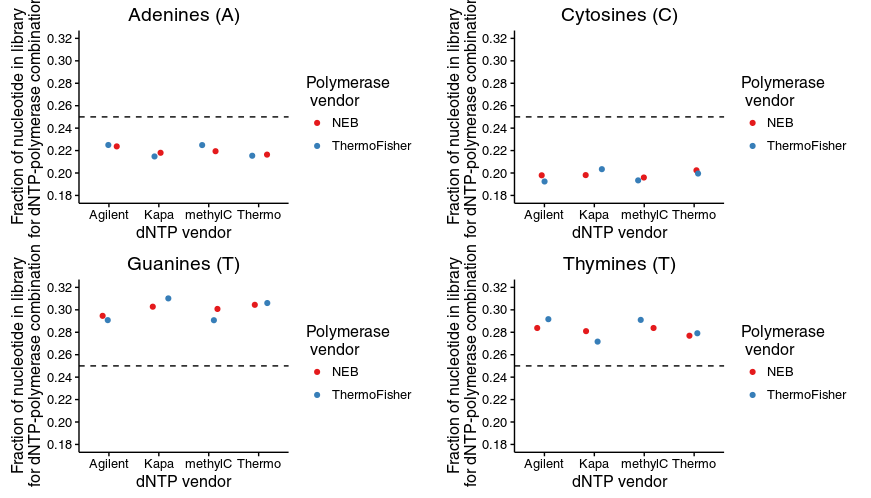
\includegraphics[width=0.8\textwidth]{linearmodel_acgt}
  \caption{Fraction of each nucleotide after 24 cycles of amplification by each combination of dNTP and Phusion High-Fidelity DNA polymerase vendors}
  \label{fig:linearmodel_nt}
\end{figure}

These fractions were then used to construct a linear model (equation~\ref{eqn:linearmodel}) with coefficients detailed in tables~\ref{tab:linearmodel_coeffs_a} and~\ref{tab:linearmodel_coeffs_b} to describe the effects of dNTP and Phusion High-Fidelity DNA polymerase vendor on the fraction of the nucleotides.

\begin{equation}
  \label{eqn:linearmodel}
  \textrm{fraction of nucleotide} \sim\ a (\textrm{enzyme vendor}) + b (\textrm{dNTP vendor}) + c
\end{equation}

\begin{table}[h]
  \centering
  \begin{tabular}{r}
     \\
    New England BioLabs\\
  \end{tabular}%
  \pgfplotstabletypeset[
  col sep = comma,
  ]{linearmodel_a.csv}  
  \caption{Coefficients for the linear model to describe the contribution of Phusion High-Fidelity DNA polymerase vendors to nucleotide fractions (`$a$' in equation~\ref{eqn:linearmodel}) for each nucleotide.  These coefficients describe increments relative to the ThermoFisher High-Fidelity DNA polymerase.}
  \label{tab:linearmodel_coeffs_a}
\end{table}

\begin{table}[h]
  \centering
  \begin{tabular}{r}
     \\
    dNTP Kapa\\
    dNTP Agilent\\
    dNTP ZymoMeC\\
  \end{tabular}%
  \pgfplotstabletypeset[
  col sep = comma,
  ]{linearmodel_b.csv}  
  \caption{Coefficients for the linear model to describe the contribution of dNTP vendors to nucleotide fractions (`$b$' in equation~\ref{eqn:linearmodel}) for each nucleotide.  These coefficients describe increments relative to the ThermoFisher dNTPs.}
  \label{tab:linearmodel_coeffs_b}
\end{table}

% This plot may go -- it doesn't add much
The predictive power of this model was verified by assessing the correlation between observed nucleotide fractions and the nucleotide fractions predicted by the linear model (figure~\ref{fig:linearmodel_ver}).  The high correlation coefficient suggested that the model had high predicting power.  Alternatively such a value is expected from the low values of linear coefficients relative to the nucleotide fractions observed.

\begin{figure}[htbp]
  \centering
  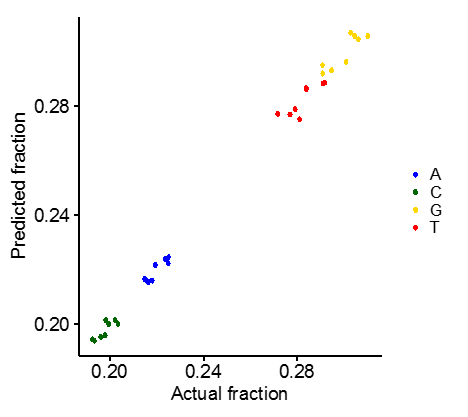
\includegraphics[width=0.4\textwidth]{linearmodel_plot}
  \caption{Verification of linear model by a scatter plot between observed fractions of each nucleotide and fractions of each nucleotide predicted by the linear model (equation~\ref{eqn:linearmodel}).  R = 0.998}
  \label{fig:linearmodel_ver}
\end{figure}

\section{Discussion}
\label{sec:pcrbias_discussion}
%% - Relevance of such bias to previous sequencing data
%% - Hints to data analysis in the future 
%% - A few discussions about Troubleshooting

All DNA polymerase enzymes tested -- Phusion, Phire, DreamTaq, and Q5  -- showed similar weak biases towards A and T.  Specifically, Phire showed the strongest bias, while Phusion showed the weakest bias.  The bottleneck effect of amplifying a small sample from a large input library was small, with Phire producing the largest bottleneck effect.  The bottleneck effect is relevant to quantification of PCR bias as it may confound patterns that arise from enzyme biases, especially if the libraries are subject to low complexity and random sampling.  Biases introduced by AMPure bead purification and reagent vendors were minimal compared to biases from DNA polymerase enzymes.

As a result, PCR bias is most likely due to the reactions in PCR themselves rather than other procedures.  Furthermore, in light of our results, when preparing a sequencing library, Phire should be avoided as it introduces the greatest PCR biases.

However, from the data it is difficult to see how much such PCR bias would contribute to procedures that employ PCR, such as nucleosome EMSA-SELEX.  The question of how much A/T bias contributes to the variances observed in the \emph{k}-mer plots remains to be solved.  Furthermore, the input library was biased towards T and G, as apparent from the measurements of nucleotide fractions in subsection~\ref{ssec:pcrbias_result_reagent} and counting nucleotide frequencies along sequencing reads in subsection~\ref{ssec:nuseqpref_fft}.  This T/G bias, likely due to the DNA synthesis process, may confound quantification of PCR bias.

Improving on these experiments would require thorough modelling work on the PCR bias and the intrinsic biases of the synthetic DNA library, followed by applying such models on the sequencing data.  Although building such a model is beyond the scope of this study, the data from this study would be useful in creating a model to predict biases introduced by PCR cycles.  PCR bias is at the same order as biases introduced by the weak affinity of the histone octamer towards specific DNA sequences.  An explicit PCR bias model would therefore be able to separate bias introduced by PCR and bias introduced by nucleosome positioning.  Such a model would lead to a better quantification of the biases introduced by nucleosome positioning.

\section{Materials and Methods}
\label{sec:pcrbias_methods}

\subsection{DNA ligand design and preparation}
\label{ssec:pcrbias_methods_lig}

The same input library (lig147) as \ref{ssec:emsaselex_methods_lig} was used, without methylation.

\subsection{Biases from DNA polymerase enzymes and bottleneck effects}
\label{ssec:pcrbias_methods_enz}

PCR amplification followed manufacturers' protocols for the following DNA polymerases: Phire Hot Start II DNA polymerase (ThermoFisher, F122S), Q5 Hot Start High-Fidelity DNA polymerase (New England BioLabs, M0493S), DreamTaq Hot Start DNA Polymerase (ThermoFisher, EP1701), and Phusion High-Fidelity DNA Polymerase (ThermoFisher, F530L).

Specifically, for each enzyme, the input library was diluted and then amplified in five experimental groups as specified:

\begin{itemize}
  \item Dilute by a factor of $2^{4}$, then amplify for 8 cycles
  \item Dilute by a factor of $2^{8}$, then amplify for 12 cycles
  \item Dilute by a factor of $2^{12}$, then amplify for 16 cycles
  \item Dilute by a factor of $2^{16}$, then amplify for 20 cycles
  \item Dilute by a factor of $2^{20}$, then amplify for 24 cycles
\end{itemize}

The amplified product for each experimental group was then sequenced.

To investigate bottleneck effects, the product from the 24-cycle amplification was diluted by a factor of $2^{20}$.  From this, two samples were taken to be amplified for 24 cycles, and then the resulting amplification product was sequenced.

\subsection{Biases from PCR cycles}
\label{ssec:pcrbias_methods_pcr}

lig147 was diluted by a factor of $2^{20}$.  PCR amplification followed manufacturer's protocols for Phusion High-Fidelity DNA Polymerase (ThermoFisher, F530L).  DNA was amplified for 4, 8, 12, 16, 20, 24, and 28 cycles, then were re-diluted so that their theoretical concentrations matched DNA amplified for 4 cycles.  The libraries for each experimental group were then sequenced.

\subsection{Biases from purification}
\label{ssec:pcrbias_methods_pur}

lig147 was purified using 1.2x AMPure beads (Beckman Coulter) according to manufacturer's protocols, but with a \SI{15}{\micro\litre} elution volume.  Purification was repeated for 1, 2, 4, and 8 times.

\subsection{Biases from reagent vendors}
\label{ssec:pcrbias_methods_reagent}

lig147 was diluted by a factor of $2^{20}$.  It was then amplified for 24 cycles using manufacturer's protocols for PCR amplification using Phusion High-Fidelity DNA Polymerase (ThermoFisher, F530L) and the reagents supplied by this vendor.

Combinations of Phusion High-Fidelity DNA Polymerase and dNTPs were investigated.  The polymerases used were from ThermoFisher (F530L) and New England BioLabs (M0530L).  The dNTPs used were from ThermoFisher (R0192), Agilent Technologies (200415-51), Kapa Biosystems (KN1009), and dNTPs containing 5-methyl dCTP in place of dCTP from Zymo Research (D1030).  Twenty-four cycles of PCR using the eight combinations of polymerases and dNTPs proceeded according to manufacturer's protocols for Phusion High-Fidelity DNA Polymerase (ThermoFisher, F530L).

\subsection{Sequencing}
\label{ssec:pcrbias_methods_seq}

The same procedures for sequencing as \ref{ssec:emsaselex_methods_seq} were used.

\subsection{Data analysis}
\label{ssec:pcrbias_methods_anal}

To investigate the effect of different vendors, a linear regression model was constructed.  The model used the frequencies of each nucleotide in the amplified library as the response variable.  The input variables were the enzyme vendor and dNTP vendor.

\backmatter

\chapter{Acknowledgements}
\label{ch:ack}

I would like to thank Prof Jussi Taipale for overseeing the project and for providing feedback regarding the experiment design and data analysis.  I also express my gratitude towards Dr Fangjie Zhu for his assistance in designing the experiments, for his mentorship throughout the project, for assistance with DNA sequencing, and for valuable feedback for this dissertation.  Lastly, I would also like to thank all members of the Taipale lab for their hospitality and general assistance.  In particular, I would like to thank Dr Otto Kauko for technical aid with the nucleosome EMSA-SELEX procedure, and Dr Minna Taipale for assistance with DNA sequencing.

\printbibliography

\end{document}